% Remember to input this to the presentative tex file before compiling.
\section{EoS from fRG}

\subsection{Polyakov-Quark-Meson (PQM) Model}

\begin{frame}
\begin{block}{Effective action:}
    \begin{align}
     \Gamma_k=&\int_x \Big\{ Z_q\,\bar{q}\big[\gamma_\mu\partial_\mu-\gamma_0(\mu+igA_0)\big]q+\frac{1}{2}Z_\phi\,(\partial_\mu\phi)^2 \nonumber\\
     &+h\,\bar{q}(T^0\sigma+i\gamma_5\vec{T}\cdot\vec{\pi})+V_k(\rho)-c\sigma+V_{\mathrm{glue}}(L,\bar{L}) \Big\}
    \end{align}
\end{block}

Here we use Local potential approximation (LPA):
\begin{align}
&\partial_tZ_{q/\phi}=0\\[2ex]
&\partial_th=0
\end{align}
We only consider a simple computation of the Grand potential.
\end{frame}
%%%%%%%%%%%%%%%%%%%%%%%%%%%%%%%%%%%%%%%%%%%%%%%%%%%%%%%%%%%%%%%%%%%%%%%%%%%%
\begin{frame}[fragile]{Effective potential}
\begin{block}{Flow equation of effective potential:}
    \begin{align}
     \partial_t V_k(\rho)=\frac{k^4}{4\pi^2}\Bigg[3\,l^{(B)}_0(m^2_\pi; T)+l^{(B)}_0(m^2_\sigma; T)-4N_cN_fl^{(F)}_0(m^2_f;\mu, T)\Bigg]
    \end{align}
\end{block}
The fermion loop for real and imaginary chemical potential
\begin{align}
    l^{(F)}_0(m^2_f;\mu, T)&=\frac{k}{3\sqrt{k^2+m^2_f}}\bigg(1-n_F(m^2_f;\mu, T;L,\bar{L})-\bar{n}_F(m^2_f;-\mu, T;L,\bar{L})\bigg)\\
    &=\frac{k}{3\sqrt{k^2+m^2_f}}\bigg(1-2\,\,\mathrm{Re}\Big(n_F(m^2_f;\mu, T;L,\bar{L})\Big)\bigg)
\end{align}
\end{frame}
%%%%%%%%%%%%%%%%%%%%%%%%%%%%%%%%%%%%%%%%%%%%%%%%%%%%%%%%%%%%%%%%%%%%%%%%%%%%
\begin{frame}[fragile]{Equation of State}
%\begin{enumerate}
    \begin{columns}
        \begin{column}{0.5\textwidth}
           \vspace{-6.5cm}
           \begin{block}{Pressure and Baryon number fluctuations:}
           \begin{align}
                p(T,\mu)=&-\Omega(\mu,T)\\[2ex]
                \chi^B_n=\frac{\partial^n}{\partial\hat{\mu}_B^n}\frac{p}{T^4},&\qquad \hat{\mu}_B=\frac{\mu_B}{T}\\[2ex]
                R^B_{m,n}=&\frac{\chi^B_m}{\chi^B_n}
           \end{align}
           \end{block}
           \hspace{0.8cm}
           \begin{itemize}
           \item The baryon number fluctuations at vanishing chemical potential can be used as Taylor coefficients
           \end{itemize}
        \end{column}
        \begin{column}{0.5\textwidth}
            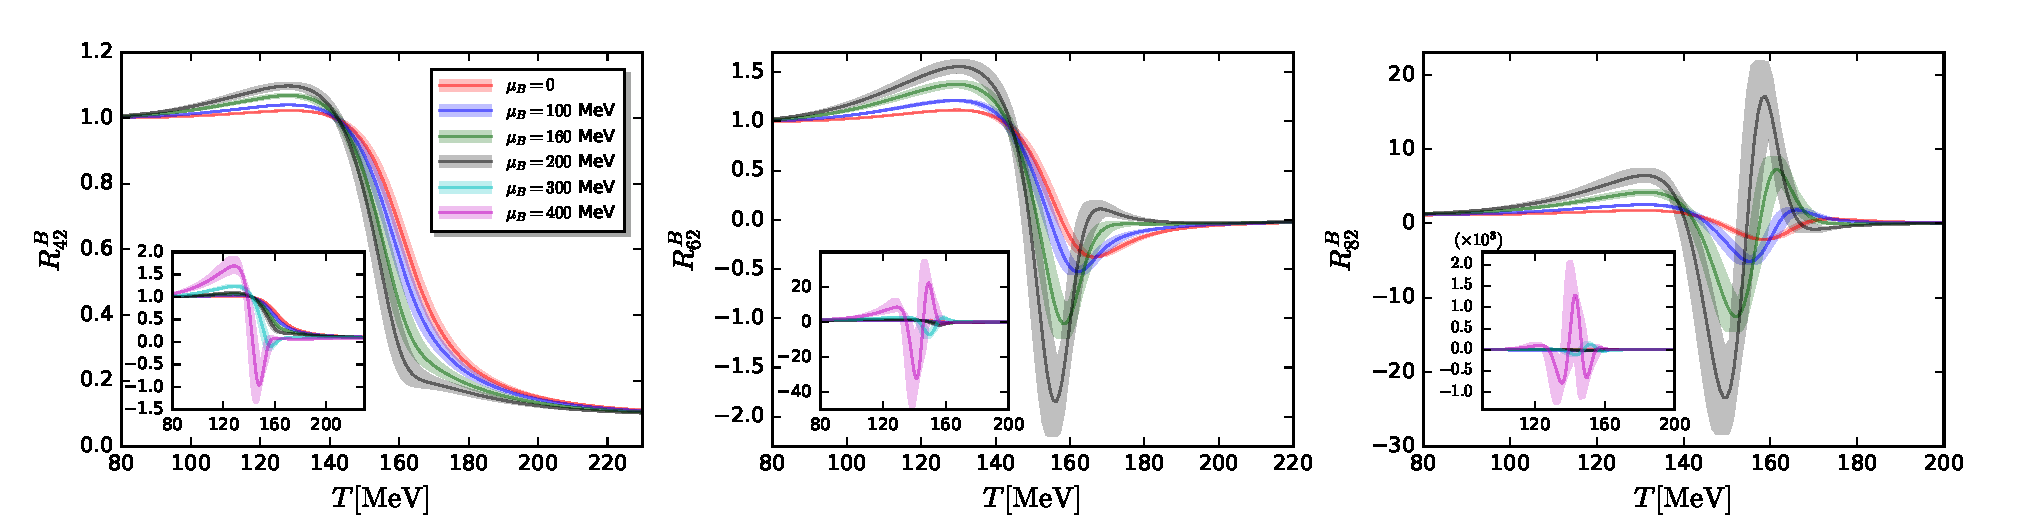
\includegraphics[width=1.\linewidth,trim={0 0 23cm 0}, clip]{Images/Figures/R42R62R82-T-muB0to400.pdf}
            \vspace{-0.8cm}
            %\hspace{0.7cm}
            \hspace{2cm}{\scriptsize Phys.Rev.D 104 (2021) 9, 094047}            
            \vspace{8cm}
        \end{column}
    \end{columns}
%\end{enumerate}
\end{frame}
%%%%%%%%%%%%%%%%%%%%%%%%%%%%%%%%%%%%%%%%%%%%%%%%%%%%%%%%%%%%%%%%%%%%%%%%%%%%
\begin{frame}[fragile]{Equation of State}
    \begin{columns}
        \begin{column}{0.5\textwidth}
           \begin{itemize}
           \item The baryon number fluctuations can be computed up to (at least) the 10th order
           \end{itemize}
        \end{column}
        \begin{column}{0.5\textwidth}
            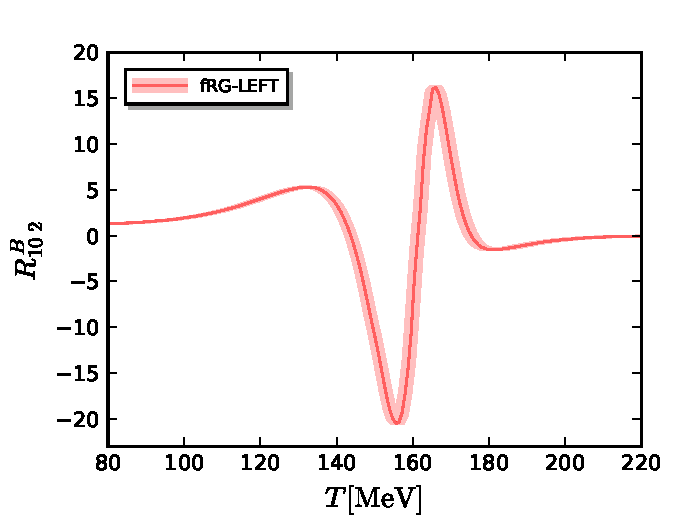
\includegraphics[width=1.\linewidth]{Images/Figures/R102-T-muB0.pdf}
            \vspace{-0.8cm}
            %\hspace{0.7cm}
            \hspace{2cm}{\scriptsize Phys.Rev.D 104 (2021) 9, 094047}            
            %\vspace{8cm}
        \end{column}
    \end{columns}
\end{frame}
%%%%%%%%%%%%%%%%%%%%%%%%%%%%%%%%%%%%%%%%%%%%%%%%%%%%%%%%%%%%%%%%%%%%%%%%%%%%
\subsection{Comparison of different Expansion methods}

\begin{frame}[fragile]
    Taylor Expansion
    \centering
    \vspace{-0.3cm}
    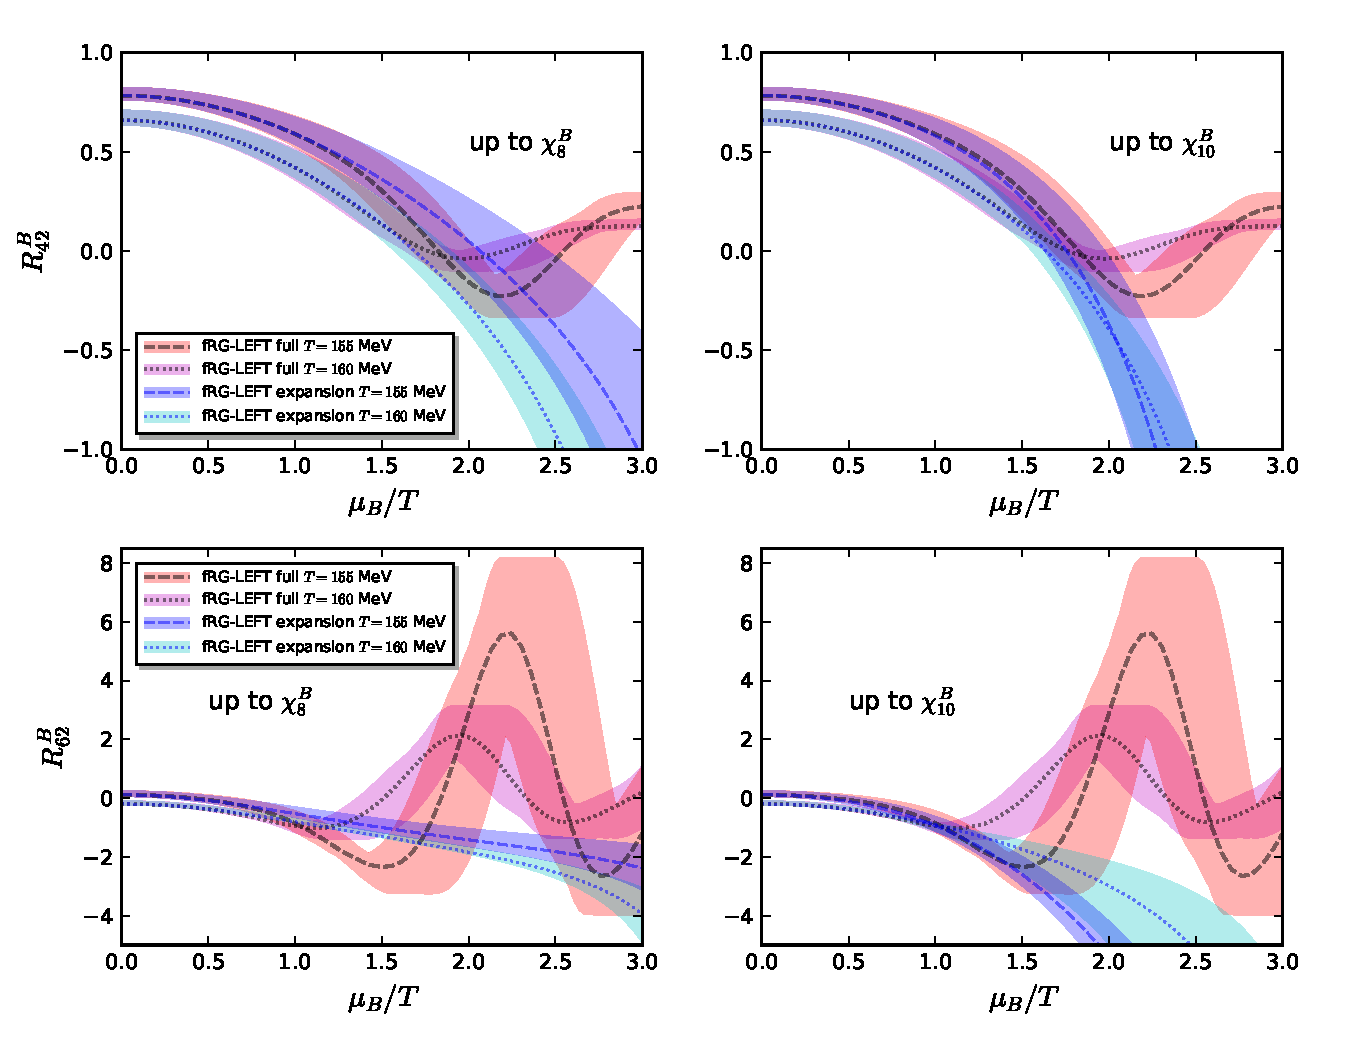
\includegraphics[width=0.9\linewidth,trim={0 9cm 0 0.5cm}, clip]{Images/Figures/R42R62expansion-muBoT.pdf}\\
    {\scriptsize Phys.Rev.D 104 (2021) 9, 094047}
    \begin{itemize}
    \item Direct calculation vs. Taylor expansion of $R^B_{42}$ \\~\
    \item The $R^B_{42}$ around $T_{pc}$ exhibits strong fluctuations at high chemical potential, which are difficult to capture with a finite-order Taylor expansion.
    \end{itemize}  
\end{frame}
%%%%%%%%%%%%%%%%%%%%%%%%%%%%%%%%%%%%%%%%%%%%%%%%%%%%%%%%%%%%%%%%%%%%%%%%%%%%
\begin{frame}[fragile]{Comparison of different Expansion methods}
    \centering
    T' Expansion
    \vspace{-0.1cm}
    \begin{columns}
        \begin{column}{0.5\textwidth}
            \includegraphics[width=0.9\linewidth]{Images/Figures/chi1_mub.pdf}
        \end{column}
        \begin{column}{0.5\textwidth}
            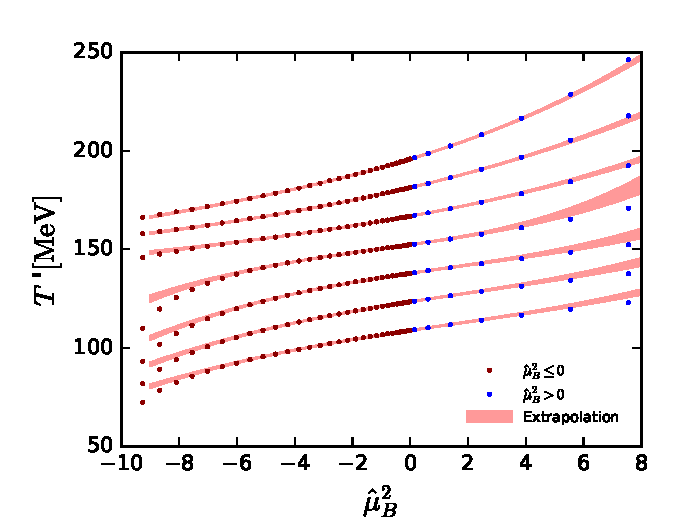
\includegraphics[width=0.9\linewidth]{Images/Figures/Ext.pdf}
        \end{column}
    \end{columns}
    {\centering \scriptsize arXiv: 2403.06770 \par}
    \begin{itemize}
    \item Directly compute at imaginary chemical potential 
    \item Apply the T’ expansion to perform extrapolation
    \end{itemize} 
\end{frame}
%%%%%%%%%%%%%%%%%%%%%%%%%%%%%%%%%%%%%%%%%%%%%%%%%%%%%%%%%%%%%%%%%%%%%%%%%%%%
\begin{frame}[fragile]{Comparison of different Expansion methods}
    \centering
    T' Expansion\\
    \vspace{-0.1cm}
    \begin{columns}
        \begin{column}{0.5\textwidth}
            \begin{align}
              T'=T\bigg( 1&+\kappa^B_2(T)\,\hat{\mu}_B^2+\kappa^B_4(T)\,\hat{\mu}_B^4\nonumber\\[2ex]
              &+\kappa^B_6(T)\,\hat{\mu}_B^6+\cdots \bigg)
            \end{align}
        \end{column}
        \begin{column}{0.5\textwidth}
            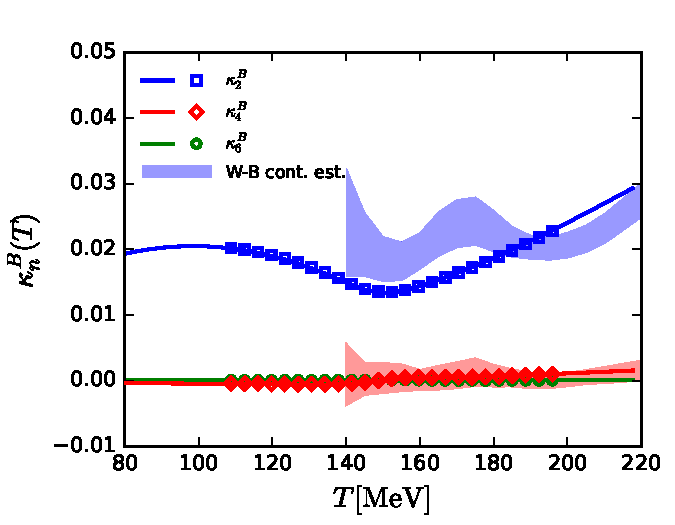
\includegraphics[width=1.\linewidth]{Images/Figures/kappa.pdf}
           {\centering \scriptsize arXiv: 2403.06770 \par}
        \end{column}
    \end{columns}
\end{frame}
%%%%%%%%%%%%%%%%%%%%%%%%%%%%%%%%%%%%%%%%%%%%%%%%%%%%%%%%%%%%%%%%%%%%%%%%%%%%
\begin{frame}[fragile]{Comparison of different Expansion methods}
    \centering
    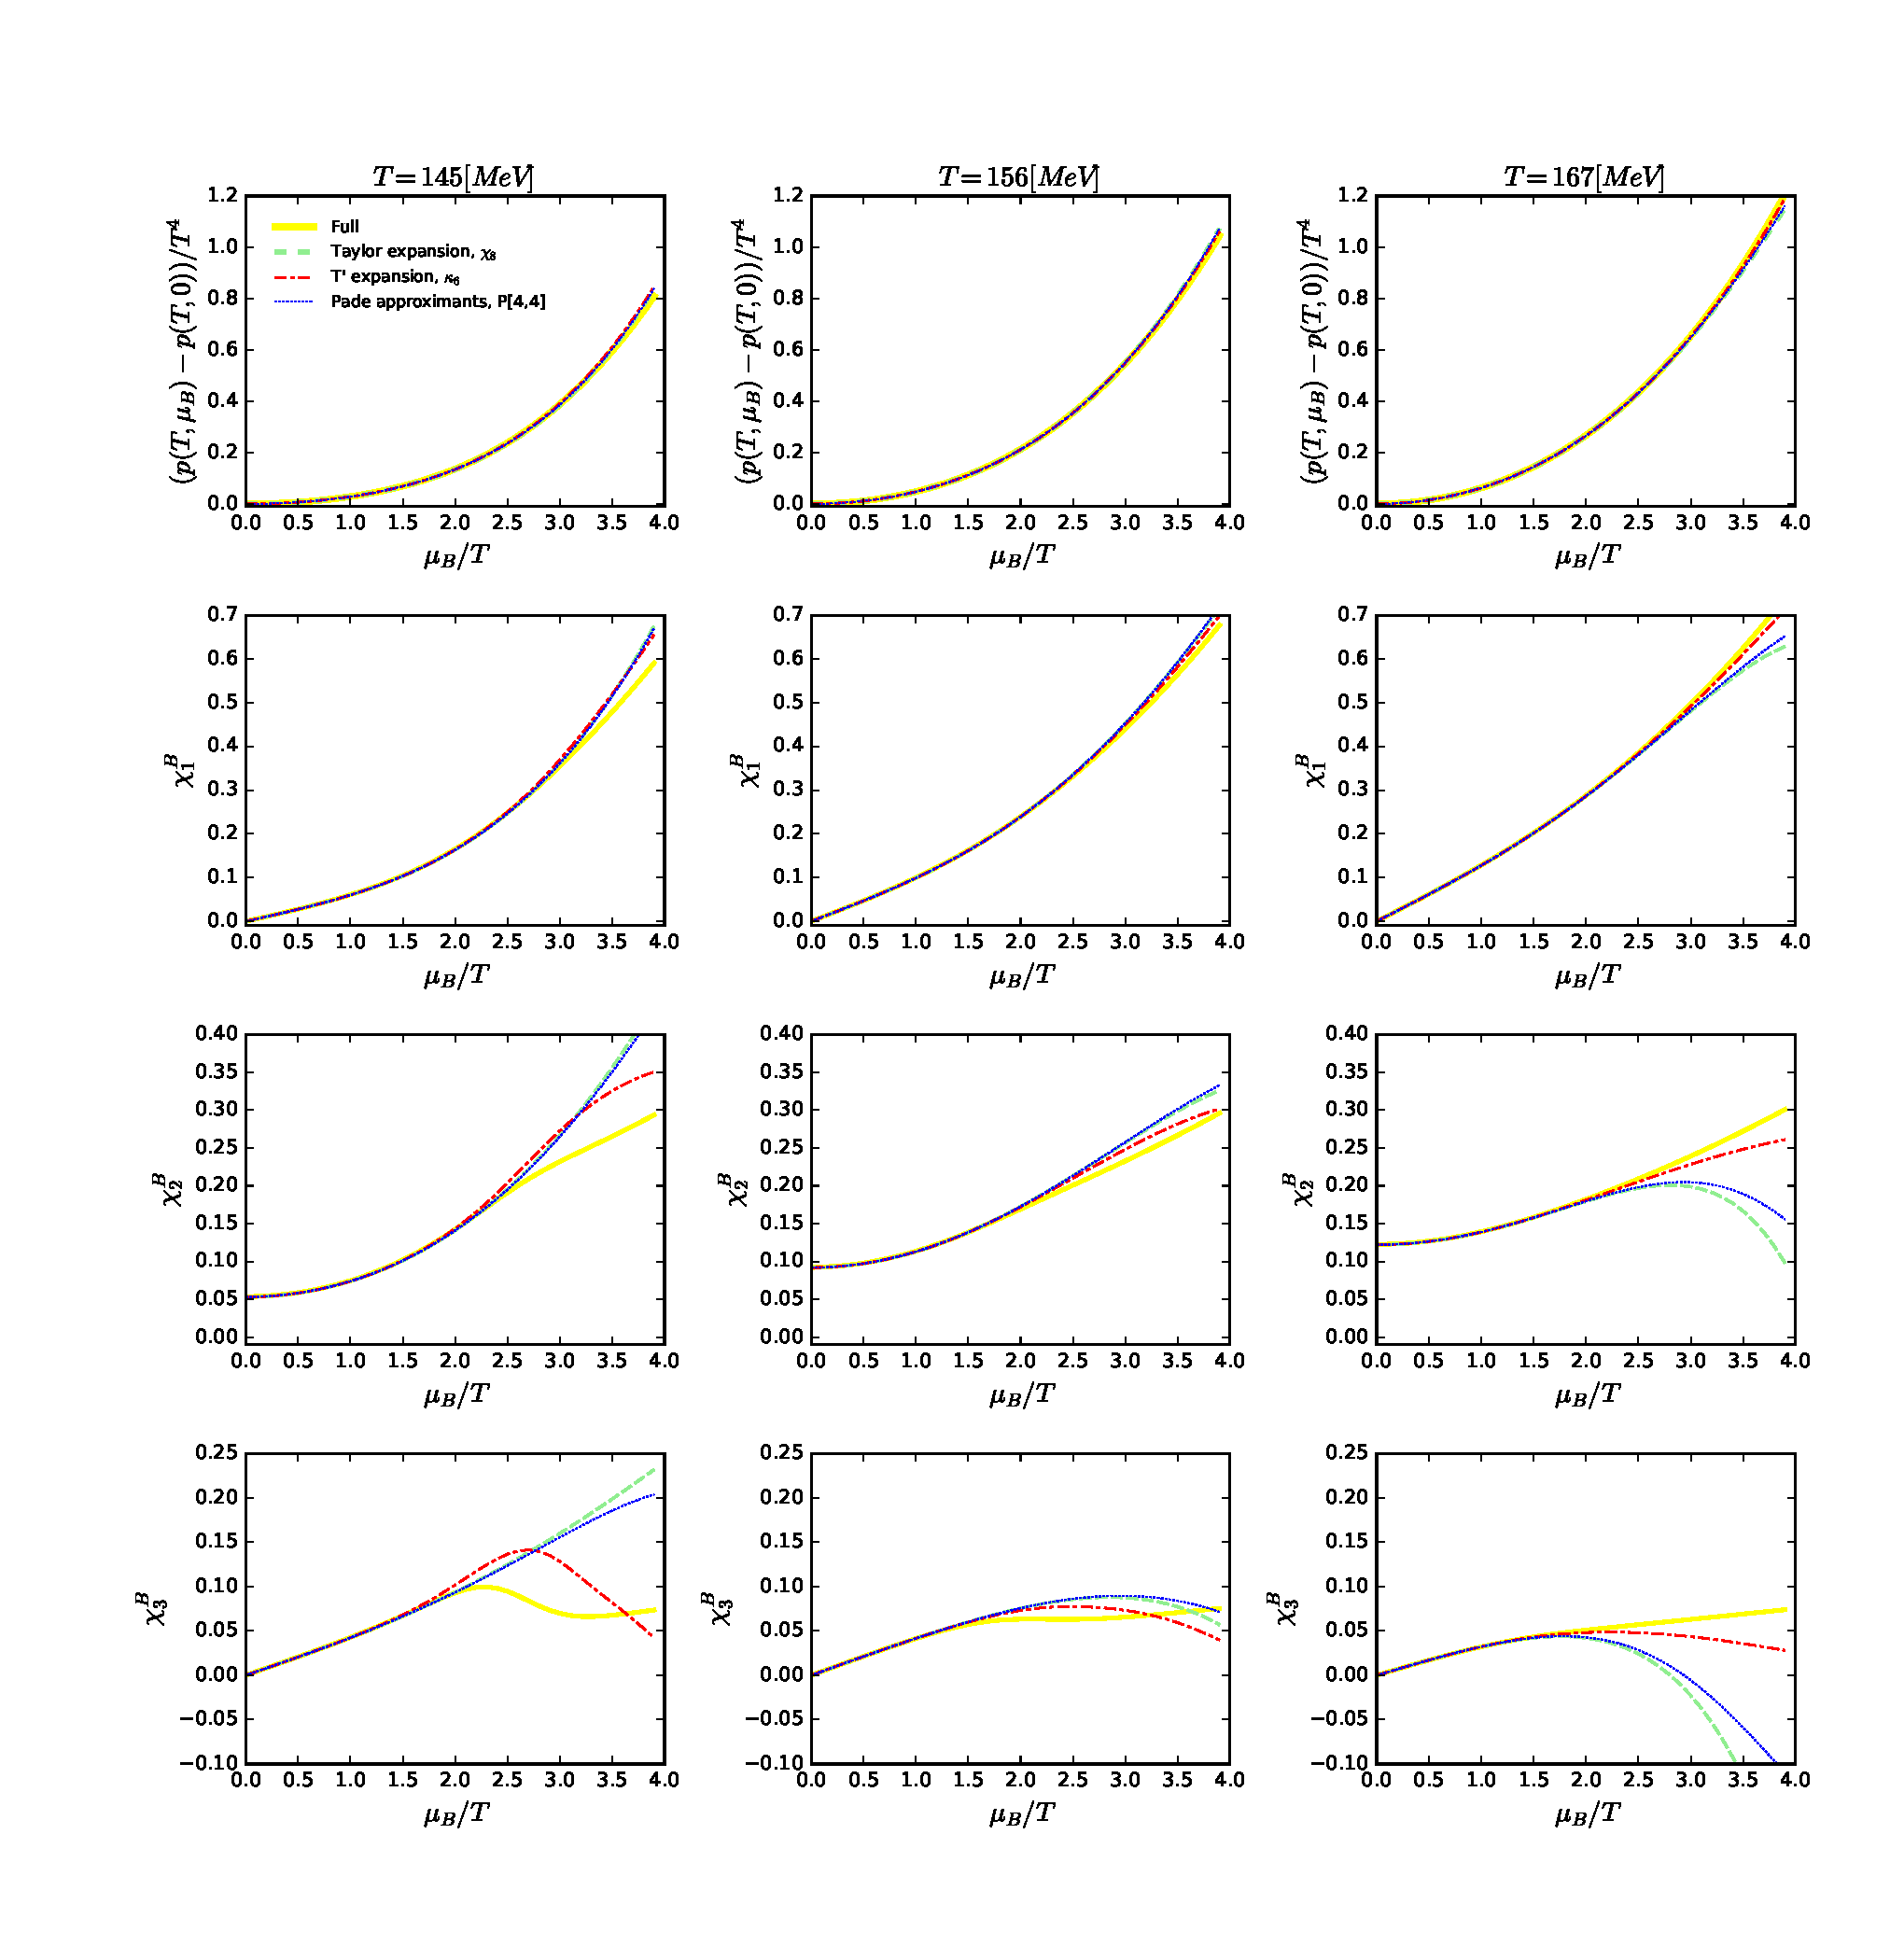
\includegraphics[width=1.\linewidth,trim={2cm 17cm 0 2.9cm}, clip]{Images/Figures/FixT.pdf}
    {\centering \scriptsize arXiv: 2403.06770 \par}
\end{frame}
%%%%%%%%%%%%%%%%%%%%%%%%%%%%%%%%%%%%%%%%%%%%%%%%%%%%%%%%%%%%%%%%%%%%%%%%%%%%
\begin{frame}[fragile]{Comparison of different Expansion methods}
    \centering
    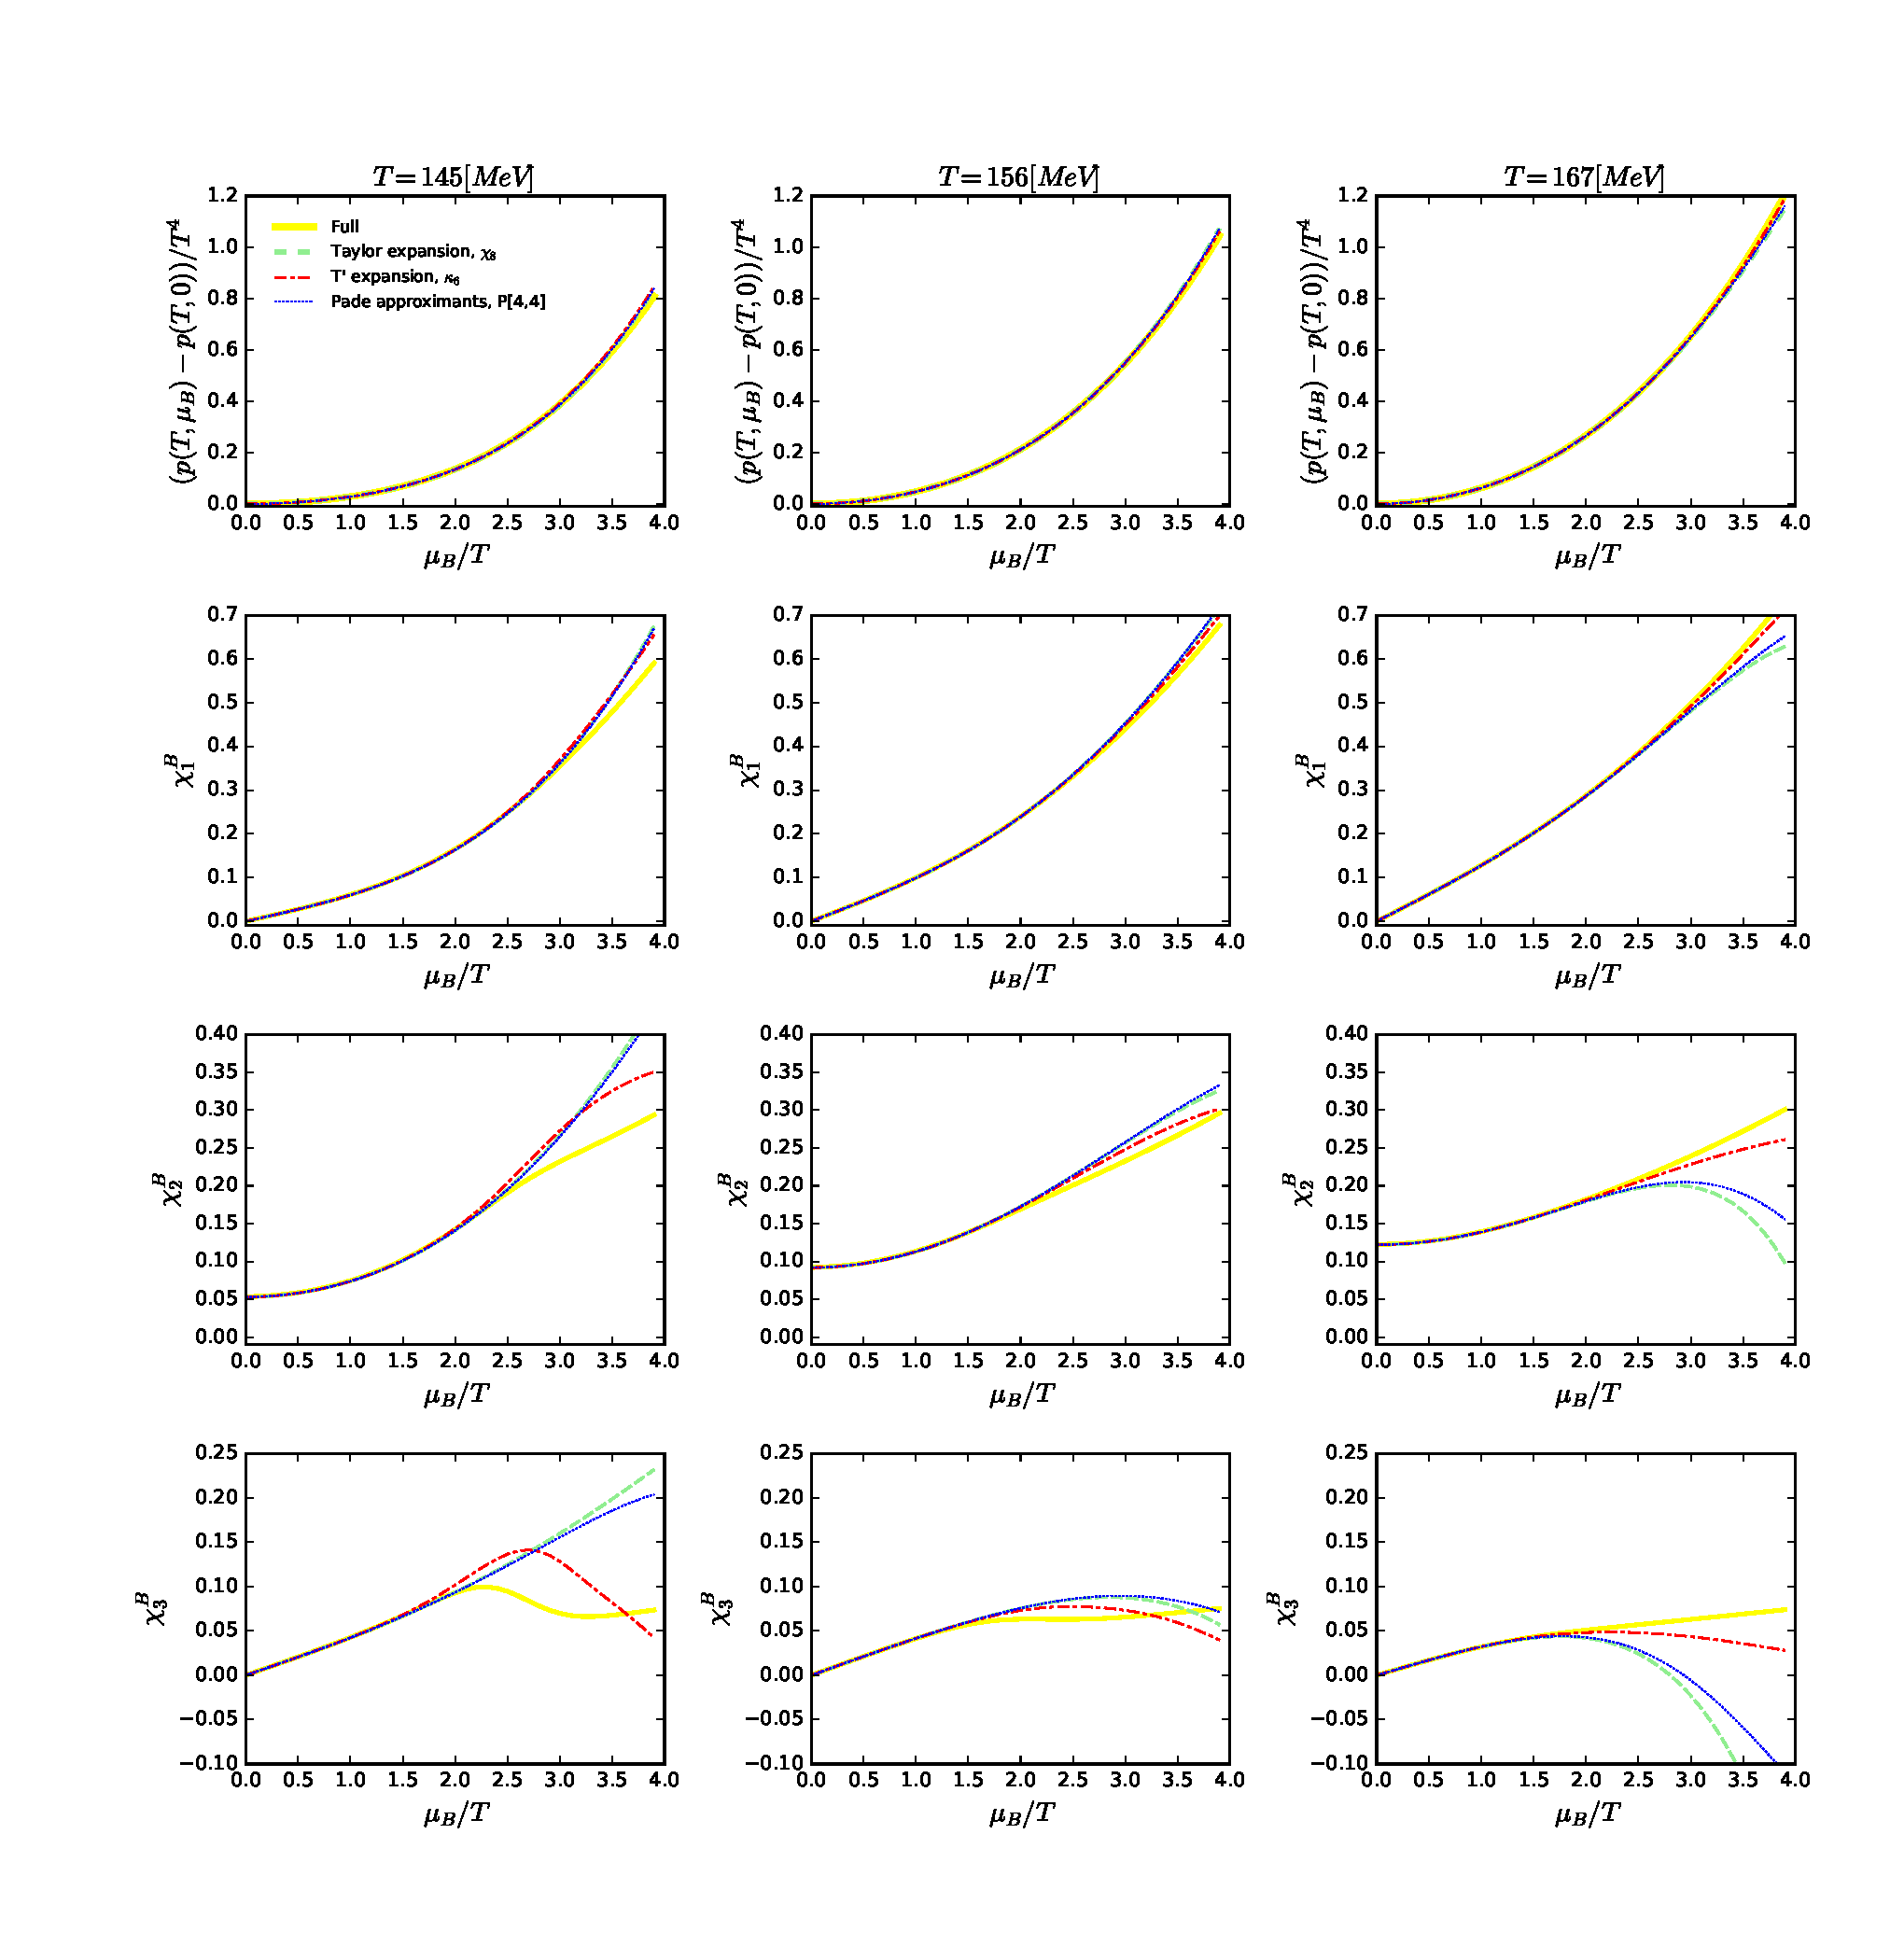
\includegraphics[width=1.\linewidth,trim={2cm 2cm 0 18cm}, clip]{Images/Figures/FixT.pdf}
    {\centering \scriptsize arXiv: 2403.06770 \par}
\end{frame}
%%%%%%%%%%%%%%%%%%%%%%%%%%%%%%%%%%%%%%%%%%%%%%%%%%%%%%%%%%%%%%%%%%%%%%%%%%%%
\begin{frame}[fragile]{Comparison of different Expansion methods}
    \centering
    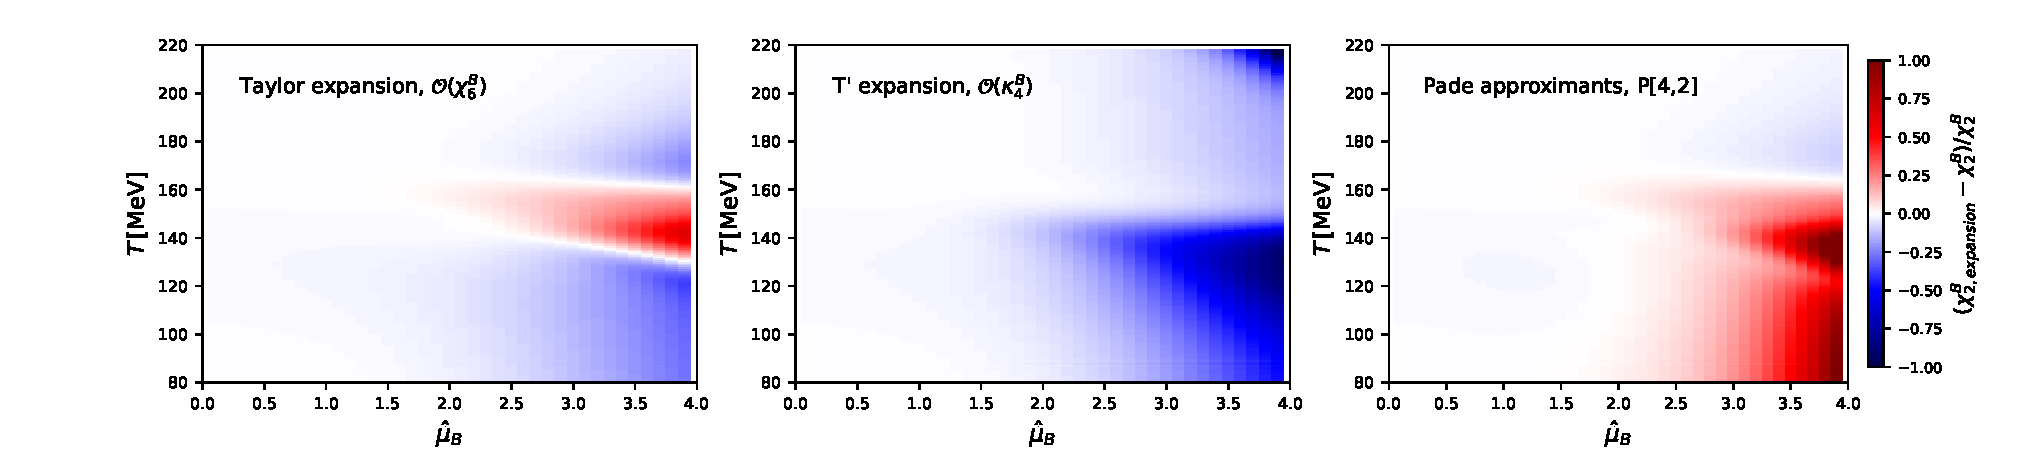
\includegraphics[width=0.87\linewidth,trim={0 0.7cm 0 0.6cm}, clip]{Images/Figures/diffchi2_3A.pdf}\\
    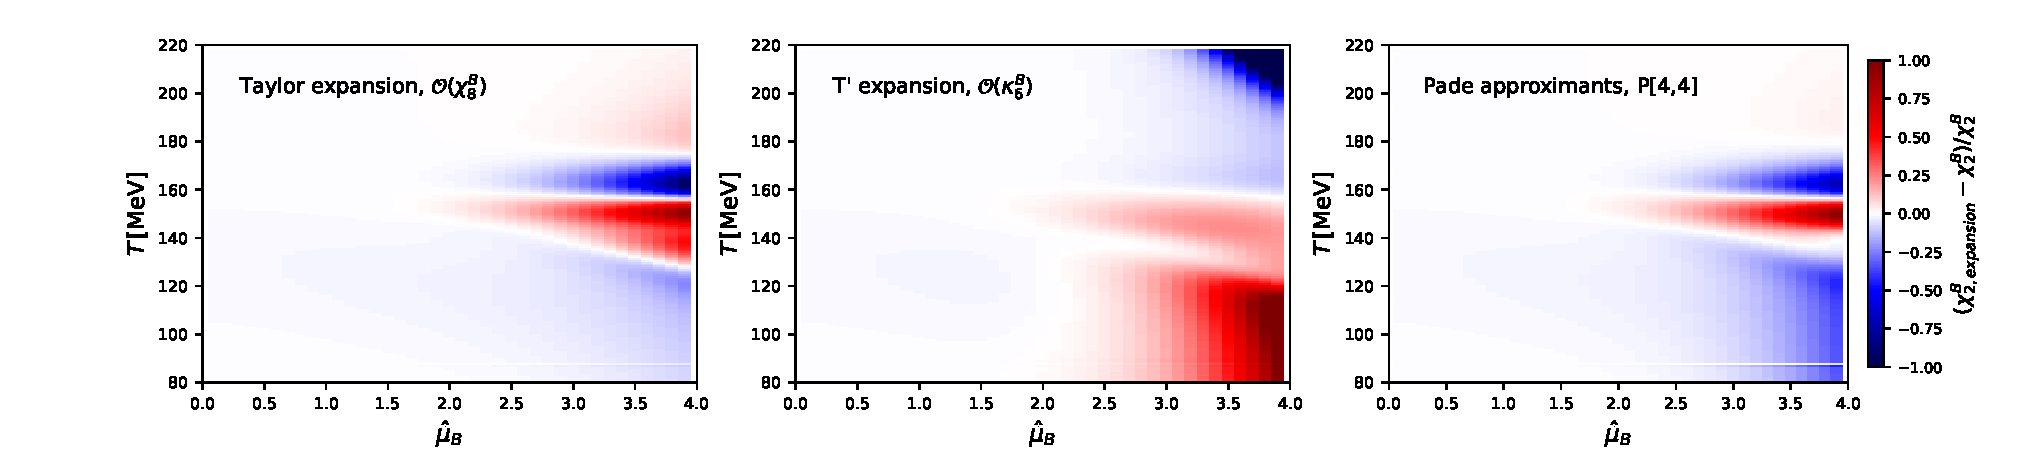
\includegraphics[width=0.87\linewidth,trim={0 0.7cm 0 0.6cm}, clip]{Images/Figures/diffchi2_3.pdf}\\
    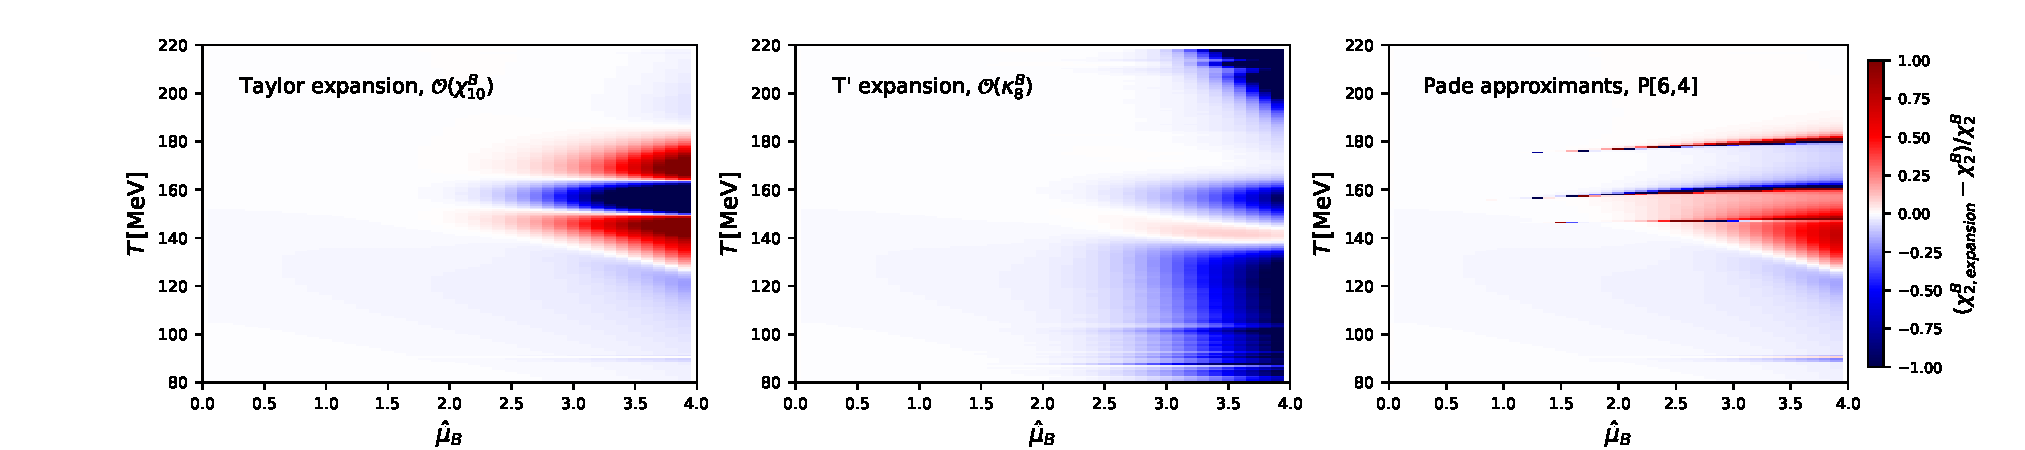
\includegraphics[width=0.87\linewidth,trim={0 0 0 0.6cm}, clip]{Images/Figures/diffchi2_3B.pdf}\\
    {\centering \scriptsize arXiv: 2403.06770 \par}
\end{frame}